% Options for packages loaded elsewhere
\PassOptionsToPackage{unicode}{hyperref}
\PassOptionsToPackage{hyphens}{url}
%
\documentclass[
]{book}
\usepackage{lmodern}
\usepackage{amssymb,amsmath}
\usepackage{ifxetex,ifluatex}
\ifnum 0\ifxetex 1\fi\ifluatex 1\fi=0 % if pdftex
  \usepackage[T1]{fontenc}
  \usepackage[utf8]{inputenc}
  \usepackage{textcomp} % provide euro and other symbols
\else % if luatex or xetex
  \usepackage{unicode-math}
  \defaultfontfeatures{Scale=MatchLowercase}
  \defaultfontfeatures[\rmfamily]{Ligatures=TeX,Scale=1}
\fi
% Use upquote if available, for straight quotes in verbatim environments
\IfFileExists{upquote.sty}{\usepackage{upquote}}{}
\IfFileExists{microtype.sty}{% use microtype if available
  \usepackage[]{microtype}
  \UseMicrotypeSet[protrusion]{basicmath} % disable protrusion for tt fonts
}{}
\makeatletter
\@ifundefined{KOMAClassName}{% if non-KOMA class
  \IfFileExists{parskip.sty}{%
    \usepackage{parskip}
  }{% else
    \setlength{\parindent}{0pt}
    \setlength{\parskip}{6pt plus 2pt minus 1pt}}
}{% if KOMA class
  \KOMAoptions{parskip=half}}
\makeatother
\usepackage{xcolor}
\IfFileExists{xurl.sty}{\usepackage{xurl}}{} % add URL line breaks if available
\IfFileExists{bookmark.sty}{\usepackage{bookmark}}{\usepackage{hyperref}}
\hypersetup{
  pdftitle={Getting Started with the Climate Adaptation Data Platform},
  pdfauthor={Brian Lee Yung Rowe},
  hidelinks,
  pdfcreator={LaTeX via pandoc}}
\urlstyle{same} % disable monospaced font for URLs
\usepackage{longtable,booktabs}
% Correct order of tables after \paragraph or \subparagraph
\usepackage{etoolbox}
\makeatletter
\patchcmd\longtable{\par}{\if@noskipsec\mbox{}\fi\par}{}{}
\makeatother
% Allow footnotes in longtable head/foot
\IfFileExists{footnotehyper.sty}{\usepackage{footnotehyper}}{\usepackage{footnote}}
\makesavenoteenv{longtable}
\usepackage{graphicx}
\makeatletter
\def\maxwidth{\ifdim\Gin@nat@width>\linewidth\linewidth\else\Gin@nat@width\fi}
\def\maxheight{\ifdim\Gin@nat@height>\textheight\textheight\else\Gin@nat@height\fi}
\makeatother
% Scale images if necessary, so that they will not overflow the page
% margins by default, and it is still possible to overwrite the defaults
% using explicit options in \includegraphics[width, height, ...]{}
\setkeys{Gin}{width=\maxwidth,height=\maxheight,keepaspectratio}
% Set default figure placement to htbp
\makeatletter
\def\fps@figure{htbp}
\makeatother
\setlength{\emergencystretch}{3em} % prevent overfull lines
\providecommand{\tightlist}{%
  \setlength{\itemsep}{0pt}\setlength{\parskip}{0pt}}
\setcounter{secnumdepth}{5}
\usepackage{booktabs}
\usepackage{amsthm}
\makeatletter
\def\thm@space@setup{%
  \thm@preskip=8pt plus 2pt minus 4pt
  \thm@postskip=\thm@preskip
}
\makeatother
\usepackage{tikz}
\usepackage{pgfplots}
\usepackage[]{natbib}
\bibliographystyle{apalike}

\title{Getting Started with the Climate Adaptation Data Platform}
\author{Brian Lee Yung Rowe}
\date{2024-06-05}

\begin{document}
\maketitle

{
\setcounter{tocdepth}{1}
\tableofcontents
}
\hypertarget{preface}{%
\chapter{Preface}\label{preface}}

We are witnessing the effects of climate change quickly accelerate.
The consequences of these changes are just starting to be felt.
To avoid widespread suffering, we need to similarly accelerate climate
adaptation initiatives.

The Climate Adaptation Data Platform (CADP) aims to do just that.
By bringing together multiple stakeholders,
we can solve multiple climate-related challenges concurrently.
This drives down costs and increases reach.

Consistent with the above goal, the CADP is an open source project.
This guide details how to use and develop the CADP.
Those wishing to contribute to the CADP should read this guide first.
Those who only want to use the CADP can skip most of the theory and focus
on the latter half of the book.

\hypertarget{license}{%
\chapter{License}\label{license}}

Copyright (C) 2024 Zato Novo, LLC.

Permission is granted to copy, distribute and/or modify this document
under the terms of the GNU Free Documentation License, Version 1.3
or any later version published by the Free Software Foundation;
with no Invariant Sections, no Front-Cover Texts, and no Back-Cover Texts.
A copy of the license is included in the section entitled ``GNU
Free Documentation License''.

\hypertarget{overview}{%
\chapter{Overview}\label{overview}}

The Climate Adaptation Data Platform (CADP) accelerates climate adaptation
initiatives by bringing together multiple stakeholders to addresss
multiple climate-related challenges.
The primary stakeholders are policymakers/governments, farmers,
and individual members of the community.
The CADP provides tangible value to each stakeholder.

The magic of the CADP is that it breaks through policy paralysis by
creating the device and data infrastructure that policymakers need to
drive widespread climate adaptation efforts.
Our hypothesis is that it's unrealistic for municipalities to deploy
and operate sensor networks.
It's also too complex an undertaking for community groups to take on.

CADP provides an alternate path where individuals and businesses purchase
devices that incrementally build out the infrastructure needed for
policymakers.

\begin{figure}

{\centering 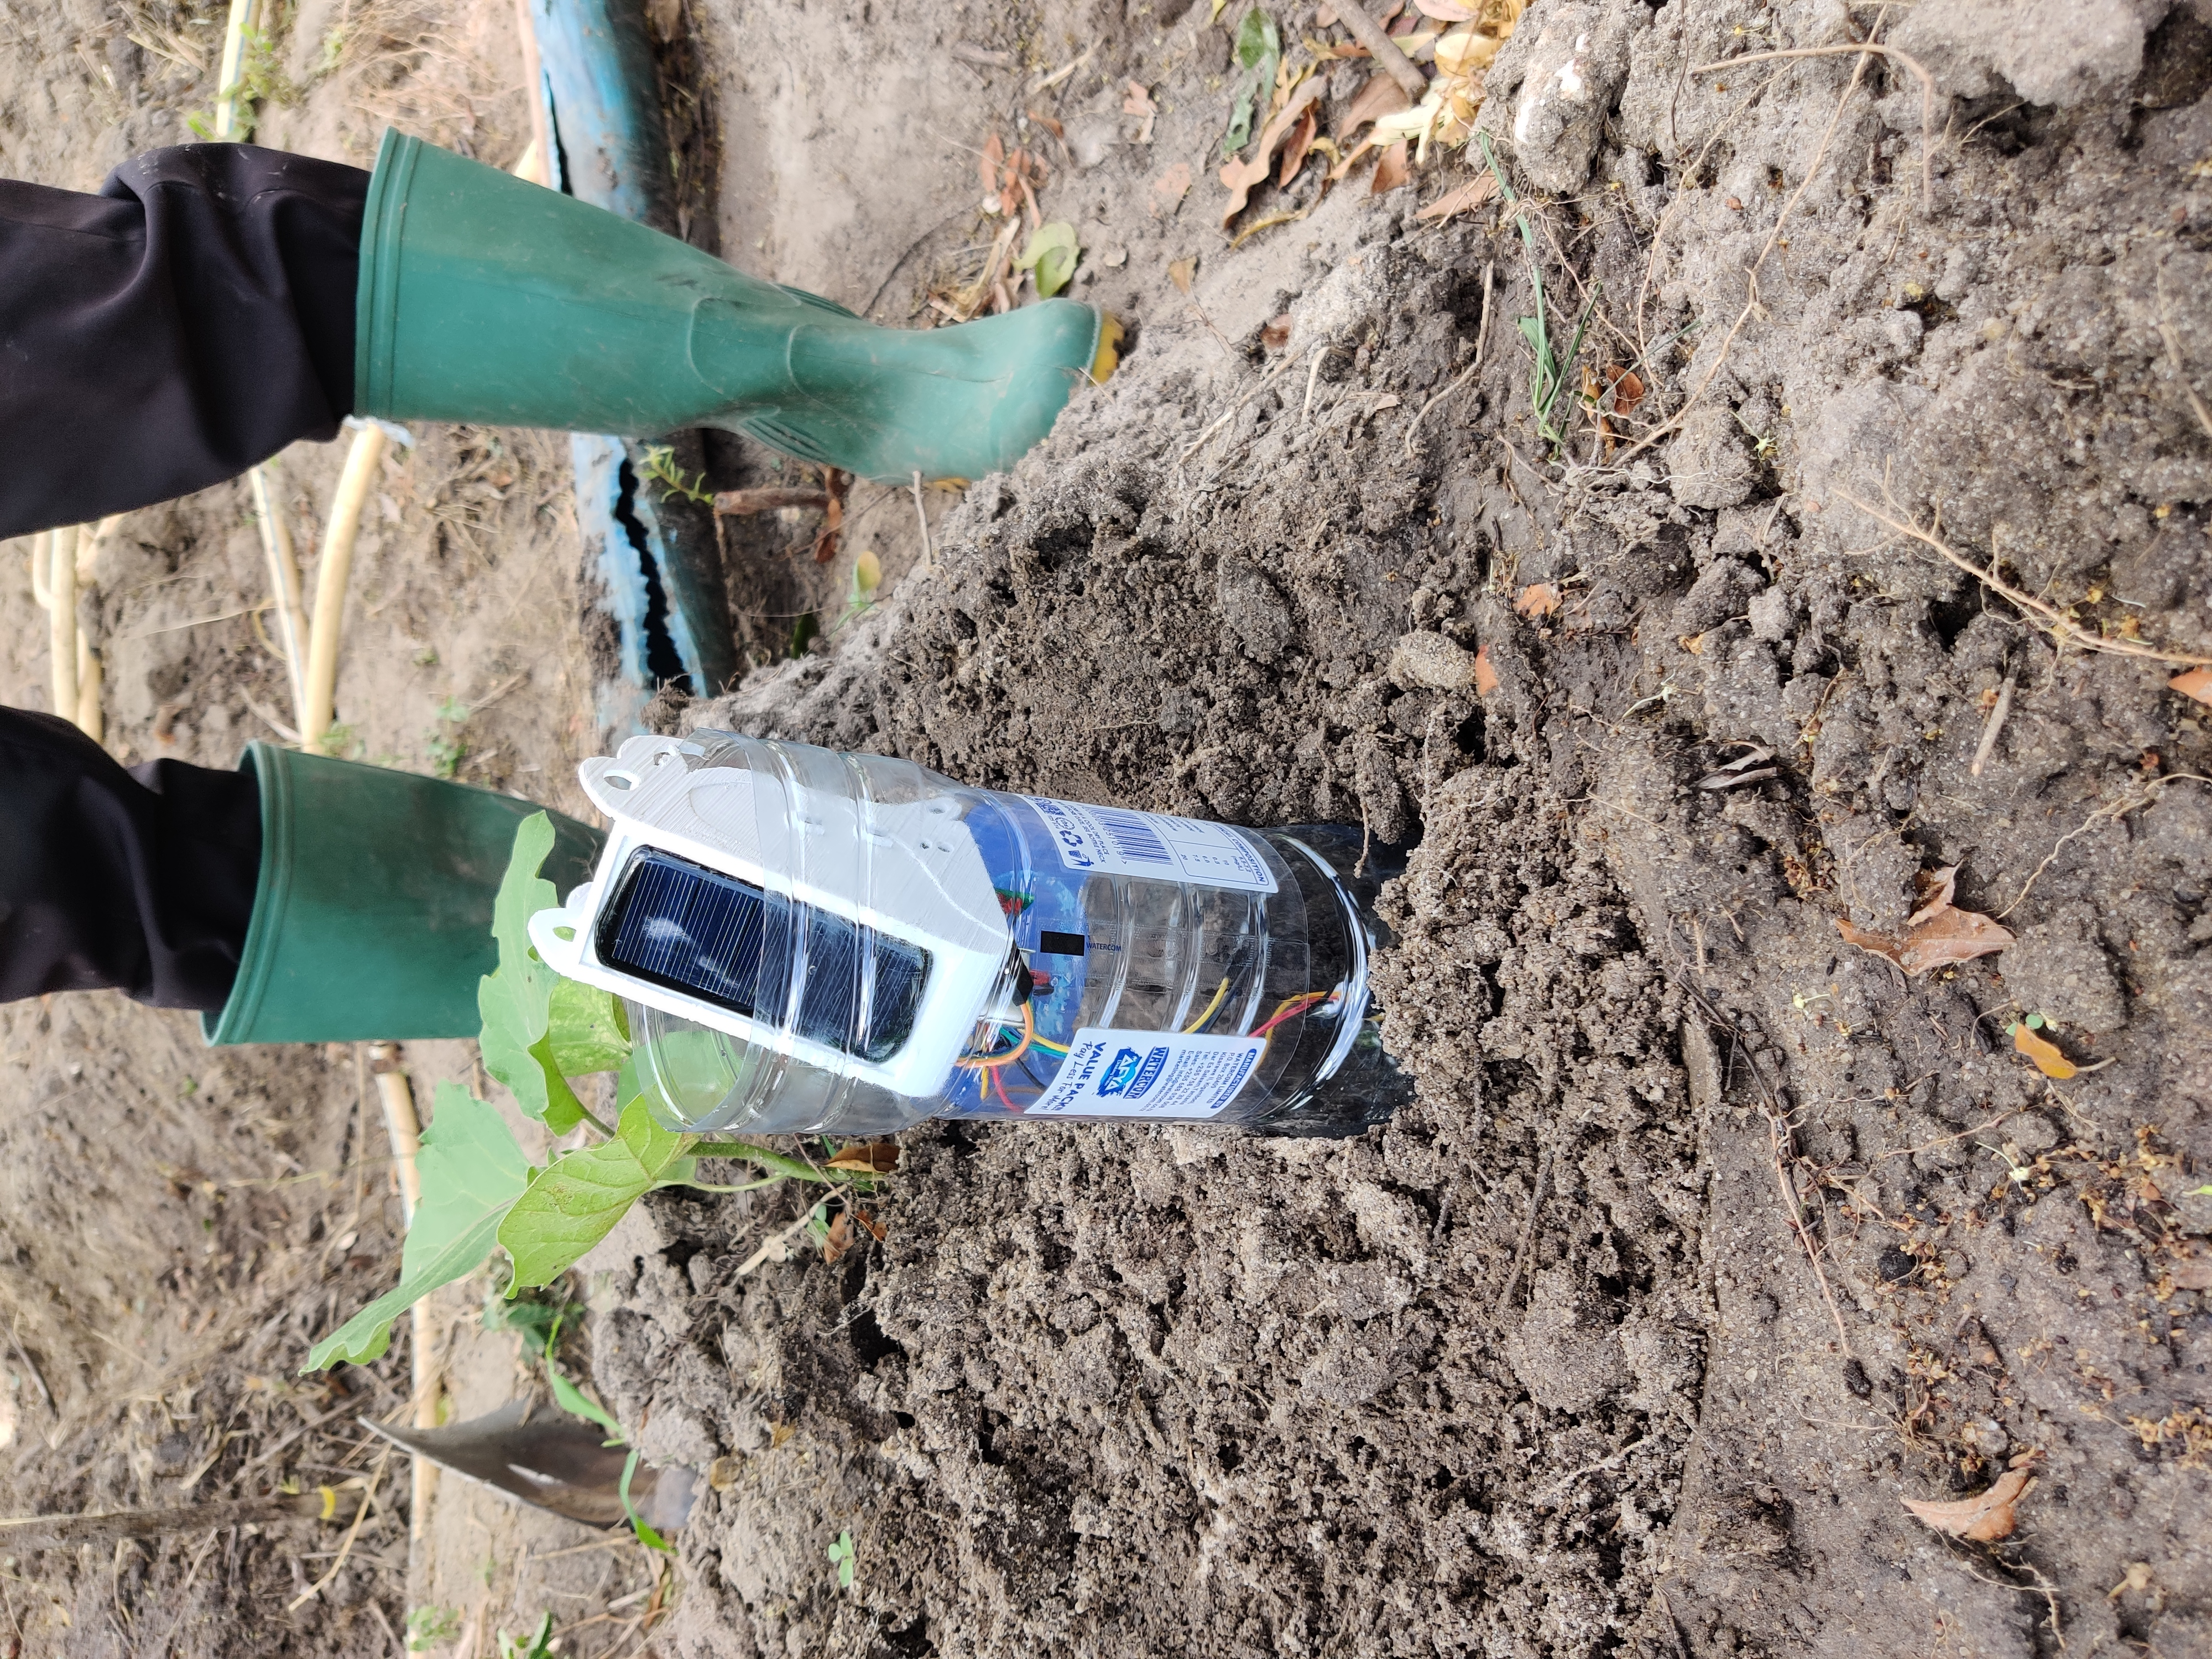
\includegraphics{images/IMG_20240223_015836} 

}

\caption{A prototype weather station device deployed at the University of Dar es Salaam test farm in Tanzania.}\label{fig:unnamed-chunk-2}
\end{figure}

This document discusses the different use cases that CADP is designed for
and the value people get from these use cases.
Where applicable, a distinction will be made between
the value individuals get from the platform versus the value policymakers get.

After describing the use cases, we move into more technical territory
so people can learn how to use and develop the platform further.
First is a high-level view of the physical infrastructure and
the relationship between a device network and the CADP.
Devices are responsible for monitoring environmental conditions
and sending the collected data to the platform.

\hypertarget{quick-start}{%
\chapter{Quick Start}\label{quick-start}}

The Climate Adaptation Data Platform is a turnkey platform for building
weather-dependent applications. CADP accelerate food security and public health
initiatives by providing all the infrastructure to automatically incorporate
hyperlocal forecasts as a data source for

\begin{itemize}
\tightlist
\item
  precision agriculture
\item
  digital advisory services
\item
  heat-health early warning systems
\item
  infectious disease early warning systems
\end{itemize}

\hypertarget{system-requirements}{%
\section{System Requirements}\label{system-requirements}}

\hypertarget{linux}{%
\subsection{Linux}\label{linux}}

The platform will work on most Debian-based Linux distributions.
At a minimum you need to have the following available:

\begin{itemize}
\tightlist
\item
  bash: this is the command line shell where you can execute commands
\item
  make: this is a standard tool to build software
\end{itemize}

In a new environment, run the \texttt{bin/init\_workstation.sh}
script to ensure you have the tools you need to build the system.

\hypertarget{windows-users}{%
\subsubsection{Windows users}\label{windows-users}}

If your primary operating system is Windows, you will need to install the
Windows Subsystem for Linux. This will give you \texttt{bash} and likely \texttt{make}.

\hypertarget{mac-users}{%
\subsubsection{Mac users}\label{mac-users}}

OS X is built on BSD. Many of the tools have slight differences from GNU Linux.
That said, the system \emph{should} run without issue on Mac OS X.

\hypertarget{docker}{%
\subsection{Docker}\label{docker}}

Docker is required. The version used to create this repo is

\begin{verbatim}
$ docker --version
Docker version 25.0.3, build 4debf41
\end{verbatim}

If you are on Windows, follow
\href{https://learn.microsoft.com/en-us/windows/wsl/tutorials/wsl-containers}{the official instructions}
for installing the Linux Subsystem for Windows and Docker desktop.

\hypertarget{building-the-platform}{%
\section{Building the Platform}\label{building-the-platform}}

The full platform can be built using the following command:

\begin{verbatim}
make all
\end{verbatim}

This will first build the platform and then launch it. The following tasks
are executed:

\begin{itemize}
\tightlist
\item
  initialize database
\item
  initialize the dashboard
\item
  build all images
\end{itemize}

You can use this command repeatedly. The \texttt{Makefile} is smart enough to know
not to re-initialize the database.

To verify that the system is running, you can check the logs or check
the container statuses directly. Logs can be monitored using \texttt{make\ logs},
while the container statuses can be viewed by typing \texttt{docker\ ps}.
In this latter command, the output should look something like this:

\begin{verbatim}
$ docker ps
CONTAINER ID   IMAGE                                                                COMMAND                  CREATED       STATUS                   PORTS                                                                                  NAMES
c86a8b8a34a2   zeomancer_system-weather_forecast                               "tini -g -- /bin/bas…"   3 hours ago   Up 3 hours (unhealthy)   443/tcp, 8888/tcp, 0.0.0.0:8180->80/tcp, :::8180->80/tcp                               zeomancer_system-weather_forecast-1
6e2812b24695   zeomancer_system-simulator_etl                                  "tini -g -- /bin/bas…"   3 hours ago   Up 3 hours (unhealthy)   80/tcp, 443/tcp, 8004/tcp, 8888/tcp, 0.0.0.0:8081->8080/tcp, :::8081->8080/tcp         zeomancer_system-simulator_etl-1
27e46eb20065   zeomancer_system-ecm_etl                                        "tini -g -- /app/zeo…"   3 hours ago   Up 3 hours (unhealthy)   80/tcp, 443/tcp, 8004/tcp, 8888/tcp, 0.0.0.0:8080->8080/tcp, :::8080->8080/tcp         zeomancer_system-ecm_etl-1
5db4dd92afa2   timescale/timescaledb:latest-pg12                                    "docker-entrypoint.s…"   3 hours ago   Up 3 hours               0.0.0.0:5432->5432/tcp, :::5432->5432/tcp                                              zeomancer_system-ts_db-1
3bb9e8c4788a   nodered/node-red:latest                                              "./entrypoint.sh"        3 hours ago   Up 3 hours (healthy)     0.0.0.0:9002->1880/tcp, :::9002->1880/tcp                                              zeomancer_system-node_red-1
dc8c438b1bf3   eclipse-mosquitto:2.0.18-openssl                                     "/docker-entrypoint.…"   3 hours ago   Up 3 hours               0.0.0.0:1883->1883/tcp, :::1883->1883/tcp, 0.0.0.0:9001->9001/tcp, :::9001->9001/tcp   zeomancer_system-mqtt_broker-1
42c737867360   gcr.io/micro-dynamo-351417/bank-transaction-classification_service   "bash"                   9 days ago    Up 9 days                8080/tcp                                                                               laughing_mendeleev
\end{verbatim}

To stop the platform, just type \texttt{make\ stop}.
You can restart the platform by running \texttt{make\ run}.
The previous state will be retained when you start back up.

\hypertarget{platform-demos}{%
\section{Platform Demos}\label{platform-demos}}

A number of demos can be deployed into your running system.

\hypertarget{get-available-demos}{%
\subsection{Get available demos}\label{get-available-demos}}

This target shows all the available demos and the regions where stations
can be loaded.

\begin{verbatim}
make list-demos
\end{verbatim}

\hypertarget{deploy-a-demo}{%
\subsection{Deploy a demo}\label{deploy-a-demo}}

Deploying a demo means that all source weather data is downloaded and loaded
into the database.
Once the source data are loaded, it is possible to run a simulation to show
how the system state evolves over time or batch run all the forecasting models
and risk rules until an arbitrary end date.
The drawback of the simulator approach is that it will take a while to
observe.

\begin{verbatim}
make run-demo
\end{verbatim}

During the installation of a demo, you will be prompted to choose whether
to continue with running batch forecasts or not.

\hypertarget{view-dashboard}{%
\subsection{View dashboard}\label{view-dashboard}}

There are two dashboard views. One defines the data processing workflows
and is for application developers. The other is for policymakers and shows
the device network and corresponding weather and application information.

\hypertarget{reset-system}{%
\subsection{Reset system}\label{reset-system}}

To run another demo, you need to reset the system state. A \texttt{make} target
makes this a simple task. Be careful: it also makes it easy to lose all your
work, since it deletes everything in the database!!

\begin{verbatim}
make reset
\end{verbatim}

\hypertarget{viewing-the-dashboard}{%
\section{Viewing the dashboard}\label{viewing-the-dashboard}}

\hypertarget{policymaker-dashboard}{%
\subsection{Policymaker dashboard}\label{policymaker-dashboard}}

The end-user reporting dashboard for decisionmakers and policymakers is
located at \texttt{http://localhost:9002/dashboard/}.

\hypertarget{system-administration-dashboard}{%
\subsection{System administration dashboard}\label{system-administration-dashboard}}

The workflows that define the processing jobs are defined in Node RED.
They are accessible at \texttt{http://localhost:9002/\#flow/}.

\hypertarget{use-cases}{%
\chapter{Use Cases}\label{use-cases}}

Every device powers multiple simultaneous use cases.
We call this use case stacking.
This is different from re-using or re-purposing a device.
With use case stacking, multiple applications run concurrently.
The supported use cases depend on the sensors attached.
The two main public health use cases only need the base set of sensors,
which means anybody with an account can get hyperlocal heat risk
and mosquito abundance information.

\begin{figure}
\centering
\includegraphics[width=.8\linewidth]{images/cadp_applications}
\caption{Use case stacking enables the CADP to power multiple simultaneous applications across public health and food security.}
\label{fig:cadp_applications}
\end{figure}

\begin{figure}
\includegraphics[width=0.9\linewidth]{_main_files/figure-latex/unnamed-chunk-3-1} \caption{The CADP provides a common infrastructure that powers multiple concurrent use cases.}\label{fig:unnamed-chunk-3}
\end{figure}

\hypertarget{public-health}{%
\section{Public health}\label{public-health}}

\hypertarget{early-warning-systems}{%
\subsection{Early warning systems}\label{early-warning-systems}}

The genesis of this project was the death of 11,000 people in Libya due
to a medicane (Mediterranean hurricane) that caused a dam to fail.
People were caught off guard because as a failed state,
Libya has no functioning weather agency.
It turns out that most of Africa has limited weather stations.
Most official weather agencies only send out seasonal forecasts.

Weather forecasts give people critical time to plan and prepare for
major weather events.
Building on top of weather forecasts are early warning systems (EWS).
These systems apply rules, or risk protocols, to forecasts to determine
the level of risk people are exposed to.
EWSes can operate on any type of forecast and includes heat risk,
air quality risk, the spread of wildfire,
the spread of infectious disease, and the spread of pests like the ash borer.

The UN declared a mandate that everyone should be covered by an early warning
system by 2030. Some \$3 billion dollars have been earmarked for this effort.
While many countries have early warning systems, many are outdated,
no longer work, or cover a limited number of risks.

The CADP provides the infrastructure to quickly build EWSes and fulfill
the UN's vision.

\hypertarget{heat-risk}{%
\subsection{Heat risk}\label{heat-risk}}

Survivability is the upper limit of temperature and humidity that humans
can withstand. Humidity has a significant impact on the maximum temperature
that humans can survive in. With high humidity, the body loses its ability
to regulate temperature via perspiration.

In some places, climate change is making heat waves more extreme and pushing
temperatures to the survivability level.
Even if that limit isn't reached, whether those conditions are livable is
another matter.
Livability limits help people understand what activities are possible
given temperature and humidity (and sun exposure).
Figure \ref{fig:livability-limits}
compares livability limits for two population
groups and whether the activity takes place in direct sun or shade.

\begin{figure}

{\centering \includegraphics[width=12.97in]{images/livability_limits} 

}

\caption{Livability limits for different METs at different temperature and humidity levels. Source: [@vanos2023]}\label{fig:livability-limits}
\end{figure}

The conversion formula between METs (\(M\)) and calories is
\begin{align}
M \frac{3.5 m}{200} = kcal/min,
\end{align}
where \(m\) is mass in kilograms.
This formula enables us to customize the heat risk of specific activities
according to each individual and their specific health conditions.

Heat risk builds on the concept of livability.
The goal is to provide an EWS that helps people understand their heat risk
exposure and make decisions about what activities to do or
how to mitigate heat risk during certain activities.
As shown in \ref{fig:cadp-ews-quebec} the platform currently highlights
risks

\begin{figure}

{\centering \includegraphics[width=12.79in]{images/cadp_ews_quebec} 

}

\caption{A screenshot of a policy dashboard showing active heat risk alerts for two devices.}\label{fig:cadp-ews-quebec}
\end{figure}

Individuals can get personalized heat risk guidance for any device in CADP.
Alerts can be delivered via email or via the mobile app.
Users can enter some health information to get better alerts.
This information is saved but
segregated from personally identifiable information (PII).

Relevant health information includes

\begin{itemize}
\tightlist
\item
  age
\item
  BMI (weight + height)
\item
  diabetes
\item
  heart issues
\end{itemize}

We envision a conversational alert message that doubles as a daily planner.
Integrating this information with preferred activities results in specific
messaging that informs people of what activities are realistic for a given
day. On a very hot and humid day, an older person may want to
limit sun exposure to an hour. That might mean that golf should be avoided,
whereas a stroll through a shaded park is more appropriate.

\hypertarget{mosquito-borne-infectious-disease}{%
\subsection{Mosquito-borne infectious disease}\label{mosquito-borne-infectious-disease}}

Mosquitos are a common disease vector and
can carry numerous infectious diseases,
such as malaria, dengue fever, zika virus, yellow fever.
Disease outbreaks are driven by the growth of a mosquito population.
To limit the severity of an outbreak,
mosquito surveillance is conducted to monitor the spread of mosquitos.
By tracking mosquito abundance, it is possible to predict how large an
outbreak might be.

Direct observation of mosquitos is an involved process.
It requires specialized devices to attract and trap mosquitos.
Usually these devices need periodic cleaning.

A simpler approach is to use a mosquito abundance model and
build risk protocols on that model.
These can be calibrated with physical traps (future).
Figure \ref{fig:mosquito-abundance-pdes} shows a system of
partial differential equations (PDEs) that describe the change
in mosquito abundance given a few parameters.
Of importance is that both temperature and humidity drive the
population growth of mosquitos.

\begin{figure}

{\centering \includegraphics[width=10.15in]{images/mosquito_abundance_pdes} 

}

\caption{A system of partial differential equations that model mosquito population growth based on environmental conditions. Source: [@erraguntla2021]}\label{fig:mosquito-abundance-pdes}
\end{figure}

We can thus use the temperature and humidity forecasts available in the CADP
to make mosquito abundance forecasts.
Figure \ref{fig:cadp-device} shows a graph of a device in the CADP.
The green line represents observational data,
while the orange time series is the forecast produced by the CADP.

\begin{figure}

{\centering \includegraphics[width=12.12in]{images/cadp_device} 

}

\caption{A device detail view showing historical temperature, a temperature forecast, plus heat risk thresholds.}\label{fig:cadp-device}
\end{figure}

\begin{enumerate}
\item Install device in observation area
\item Enable mosquito abundance alerts
\end{enumerate}

\hypertarget{precision-agriculture}{%
\section{Precision agriculture}\label{precision-agriculture}}

Helping farmers in Africa was the genesis of this project.
The CADP has the potential to accelerate precision agriculture initiatives.
Precision agriculture can increase crop yields and protect against
drought (food security) by conserving water usage.

Reducing water usage also improves public health.
Many areas rely on rain water as their primary potable water source.
That means irrigation is often competing with personal hydration for water.
Optimizing water usage means there can be sufficient water for both needs.

\begin{figure}

{\centering 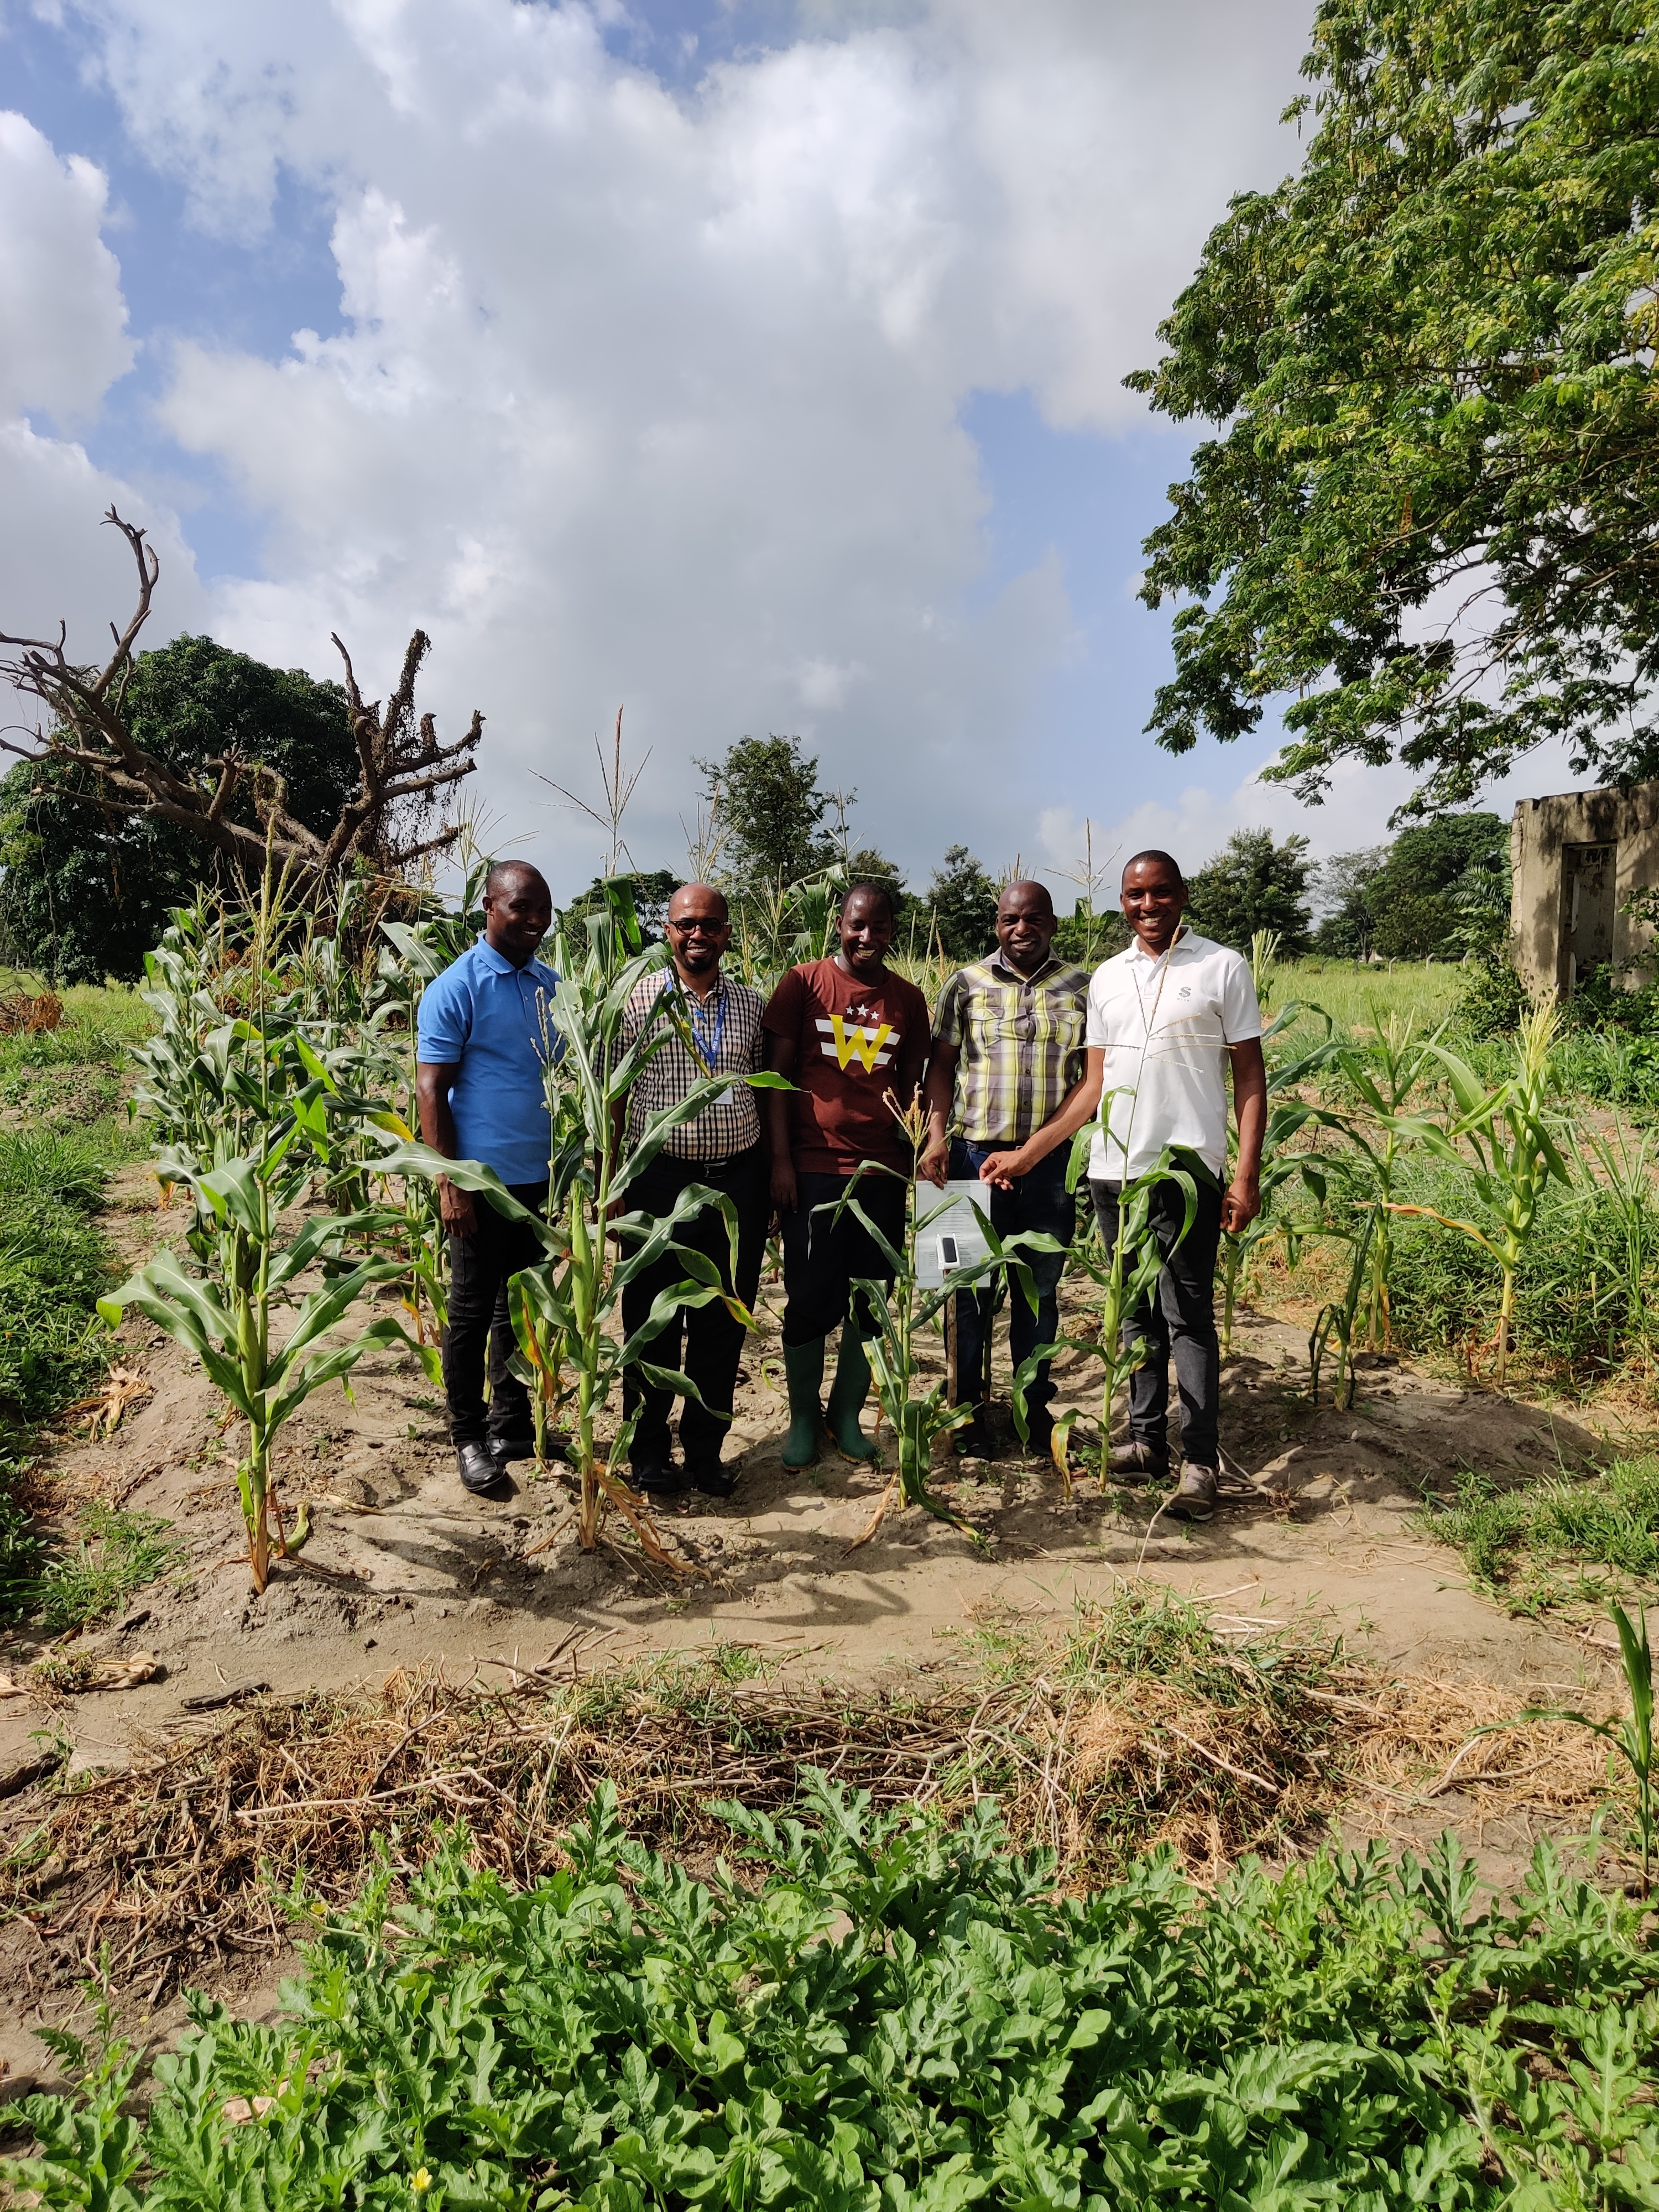
\includegraphics{images/IMG_20240220_013145} 

}

\caption{UDSM professors and agronomy staff standing behind a prototype weather station device.}\label{fig:unnamed-chunk-4}
\end{figure}

Precision agriculture is a complex field.
Our aim is to simplify the process and reduce its cost to make it accessible
to smallholder farmers worldwide.

We phase in the approach with the following steps:

\begin{itemize}
\tightlist
\item
  dry soil forecasting
\item
  watering schedules
\item
  crop calendars
\item
  risk protocols
\item
  irrigation control
\end{itemize}

\hypertarget{dry-soil-forecasting}{%
\subsection{Dry soil forecasting}\label{dry-soil-forecasting}}

Forecasting dry soil is the first step in irrigation control.
Soil that is either too dry or too wet can be harmful to plants.
While the optimal amount of water is specific to each plant,
preventing over and underwatering can be accomplished simply by monitoring
soil moisture.

A soil moisture forecast can notify the farmer or gardener when soil needs
watering.
By waiting for a watering signal, this approach avoids overwatering,
which conserves water.

The deployment model shown in Figure \ref{fig:precision-ag-1} is relatively
simple. A single sensor device is required that has a soil moisture sensor
attached to it.

\begin{figure}

{\centering \includegraphics[width=13.33in]{images/precision_ag_1} 

}

\caption{A simple installation where a single device monitors soil moisture for a crop.}\label{fig:precision-ag-1}
\end{figure}

\hypertarget{crop-watering-needs}{%
\subsection{Crop watering needs}\label{crop-watering-needs}}

Watering depends on the type of plant growing. Some plants need a lot of water while others don't. Many plants don't like wet roots, so watering cannot be too frequent. We need to develop these control models for each plant.

Water needs change based on the maturity of the plant. Beans need moist soil when pods are forming. To form large roots, beets need minimal water during early growth stages to promote root development.

We can extract this data from various agricultural sites, such as the Farmers Almanac. The information needs to be encoded into programmatic rules.

Crop calendars show the planting season and duration for different regions.

\begin{figure}

{\centering \includegraphics[width=8.33in]{images/eafrica_ke_calendar} 

}

\caption{Crop calendars for Kenya. Source: [@usda1]}\label{fig:unnamed-chunk-5}
\end{figure}

We use the approach defined by \citet{brouwer1986} that determines water need
based on evapotranspiration \(ET_o\) and a crop factor \(K_c\).

TODO: Incorporate information from this webpage:
\url{https://www.fao.org/4/s2022e/s2022e07.htm\#3.2.4\%20determination\%20of\%20crop\%20factors}

\hypertarget{risk-protocol-for-dry-soil}{%
\subsection{Risk protocol for dry soil}\label{risk-protocol-for-dry-soil}}

Knowing whether soil needs irrigation depends on a few factors. First, the crop determines the general watering schedule. Decisions are made based on reconciling watering needs with current environmental conditions. We need to know the current soil moisture level. We also want to know the future soil moisture level, which factors in weather forecasts. There's no point watering today if it will rain tomorrow.

\hypertarget{irrigation-control}{%
\subsection{Irrigation control}\label{irrigation-control}}

Automated irrigation control builds on top of the water needs forecasting model.

\begin{figure}

{\centering \includegraphics[width=13.33in]{images/precision_ag_2} 

}

\caption{A more sophisticated system with a separate device that controls an irrigation pump.}\label{fig:precision-ag-2}
\end{figure}

\hypertarget{freeze-warnings}{%
\subsection{Freeze warnings}\label{freeze-warnings}}

Farmers and gardeners in temperate or similar climates
need to know when there are frosts that could damage fragile seedlings.
Uncertainty leads to wasted time preparing for non-events or
stress worrying about whether plants will be okay.

Crop tables typically show temperature ranges that specific crops can tolerate.

\begin{figure}

{\centering \includegraphics{images/crop_temperature_guide} 

}

\caption{Planting guides for different vegetables}\label{fig:unnamed-chunk-6}
\end{figure}

\hypertarget{hotter-times}{%
\section{Hotter Times}\label{hotter-times}}

This site is used to display public data related to the sensor network.
Hotter Times thus becomes a public service where everyone can benefit from
the device network.

All of the layers discussed above can be displayed on Hotter Times.

\hypertarget{physical-infrastructure}{%
\chapter{Physical Infrastructure}\label{physical-infrastructure}}

Devices can connect with the CADP via different means.
Figure \ref{fig:device-networking} shows two different approaches.
The simplest approach is to connect directly via WiFi.
In this approach, a device communicates directly with the CADP MQTT server.
This approach works well when reliable WiFi is available.

\begin{figure}

{\centering \includegraphics[width=19.99in]{images/device_networking} 

}

\caption{Different network configuration of system.}\label{fig:device-networking}
\end{figure}

The method used for remote areas with limited infastructure utilizes
a mobile phone as an intermediary.
In this approach we assume that mobile phones (with a network connection)
exist in proximity to devices but they are no fixed internet gateways.
We call the mobile phones ephemeral gateways because they may disappear
at any time.

Ephemeral gateways (EGs) offer a temporary network connection.
The EG is responsible for pushing data to the CADP MQTT server.
If a network connection is unavailable,
it will cache the data on the mobile phone until a network connection is
available.
Once a connection is established, the EG must push the data to the server.

Devices are connected together via the LoRa wireless protocol.
When a particular device connects with an ephemeral gateway,
it broadcasts a message to other connected devices and notifies them
that it has a network connection.
This device will attempt to upload as much data to the mobile device as
possible.

Devices that receive this message will begin broadcasting data to be received
by the device connected to the EG.
The broadcast includes the ID of the device connected to the EG.
Only the device connected to the EG can broadcast an ack back.

In the event that multiple EGs are available,
each device is responsible for choosing the device to use as the target EG.

\hypertarget{direct-wifi-connections}{%
\section{Direct WiFi connections}\label{direct-wifi-connections}}

Devices connected via WiFi will start a MQTT client to send directly to
the cloud MQTT broker.
By default, the MQTT broker host is \texttt{mqtt.zeomancer.com}.

\hypertarget{ble-connections}{%
\section{BLE connections}\label{ble-connections}}

When a smartphone connects to a device via BLE, a few things happen:

\begin{itemize}
\tightlist
\item
  the device sends a test data packet to confirm that data is sent to the MQTT broker
\item
  the device waits for an ack from the smartphone
\item
  if successful,

  \begin{itemize}
  \tightlist
  \item
    LoRa is activated
  \item
    a \texttt{internet\_available} message is broadcast over LoRa
  \end{itemize}
\end{itemize}

\hypertarget{data-routing-algorithm}{%
\subsection{Data routing algorithm}\label{data-routing-algorithm}}

The data routing algorithm solves one key problem, which is the existence
of ephemeral gateways.
Devices are connected to each other via LoRa.
The goal is to efficiently route data through the LoRa network to
devices that are connected to the network (a ``connected device'').
LoRa works via a broadcast mechanism, so devices are either
in range or out of range of a connected device.

If a device is in range, then the device simply broadcasts its data to
the target connected device.
Any other device that receives the message will ignore the message
if the target id does not match its device id.

For a device that is out of range, it will send data to the nearest device
in range of a connected device.
The devices can be modeled as a graph where each device is a node
and edges represent the signal strength between them.
We can define two relevant distance metrics between two arbitrary nodes:

\begin{itemize}
\tightlist
\item
  the number of edges (aka hops) between nodes;
\item
  the harmonic mean of the signal strength of the edges separating the nodes.
\end{itemize}

A device chooses a target device by considering the harmonic mean of
the signal strengths between it and a connected device.
Generally, the device should choose the path with the highest value.
Note that this may change as EGs can move around and disappear altogether.

\hypertarget{mobile-app}{%
\chapter{Mobile app}\label{mobile-app}}

A mobile application is used to mediate the network connection for devices
in remote areas. It is also used to deliver alerts to users.
Using the device as an alert delivery mechanism ensures users have the device
installed and able to act as a data transport for devices.

\hypertarget{device-operation}{%
\chapter{Device Operation}\label{device-operation}}

Devices are designed to work with minimal configuration.
Even if you have a fixed WiFi connection available,
it is simplest to configure the device via your smartphone.

The basic steps are:

\begin{itemize}
\tightlist
\item
  install device in activity area
\item
  pair device via Bluetooth
\item
  configure device via app

  \begin{itemize}
  \tightlist
  \item
    set location
  \item
    (optional) configure and enable WiFi
  \end{itemize}
\end{itemize}

\hypertarget{components}{%
\section{Components}\label{components}}

The following information is provided in the event that repairs need to be
made to a device.

\hypertarget{connectors}{%
\subsection{Connectors}\label{connectors}}

\begin{itemize}
\tightlist
\item
  Molex 51005-2P connector for LiPo batteries
\end{itemize}

\hypertarget{cadp-architecture}{%
\chapter{CADP Architecture}\label{cadp-architecture}}

The architecture of the CADP comprises:

\begin{itemize}
\tightlist
\item
  a low power and long range sensor devices;
\item
  a data collection and storage facility;
\item
  a pluggable predictive models for producing forecasts and predictions;
\item
  a reporting dashboard for decisionmakers and policymakers; and
\item
  a delivery mechanism to provide alerts and suggested interventions to individual stakeholders.
\end{itemize}

\begin{figure}

{\centering \includegraphics[width=19.33in]{images/infrastructure_deployments} 

}

\caption{System architecture to generate weather forecasts and monitor devices.}\label{fig:infrastructure-deployments}
\end{figure}

The system has two primary sources of data. The first is baseline
weather forecast data, produced by the European Center for Medium-range
Weather Forecasts (ECMWF).
This is a global, gridded dataset with 0.4 degree resolution.
These forecasts are archived in Amazon S3 and are publicly accessible.

The second dataset comes from the devices themselves. The sensor data is
used to tune the gridded forecast according to local conditions.

\hypertarget{design-principles}{%
\section{Design principles}\label{design-principles}}

\begin{itemize}
\tightlist
\item
  Plan for 18 month shelf life
\item
  Focus on end-to-end infrastructure
\item
  Stub components where necessary
\item
  Use concurrency where appropriate to minimize wall time
\item
  Minimize data movement
\item
  Minimize cost
\end{itemize}

\hypertarget{database}{%
\section{Database}\label{database}}

\hypertarget{sensor-data-ingestion}{%
\section{Sensor data ingestion}\label{sensor-data-ingestion}}

\hypertarget{raw-sensor-data}{%
\subsection{Raw sensor data}\label{raw-sensor-data}}

Stored as an unnormalized delimited file.
These files have no header, and each row is self-contained.

The general format of the file is \texttt{key,timestamp,values},
where \texttt{values} represents an arbitrary number of additional fields.

For example, the following snippet shows actual sensor data in this format.

\begin{verbatim}
air_t_h_p,2024-01-15T00:03:26,-5.34,85.30,1048.80
battery,2024-01-15T00:08:23,0.8398108
air_t_h_p,2024-01-15T00:13:20,-5.19,83.84,1049.22
air_t_h_p,2024-01-15T00:23:15,-5.11,82.51,1049.31
battery,2024-01-15T00:28:12,0.8361486
air_t_h_p,2024-01-15T00:33:09,-6.98,83.39,1049.73
air_t_h_p,2024-01-15T00:43:03,-6.97,82.98,1050.29
battery,2024-01-15T00:48:00,0.8359045
air_t_h_p,2024-01-15T00:52:57,-6.99,84.48,1050.52
air_t_h_p,2024-01-15T00:57:44,-5.05,84.28,1050.53
battery,2024-01-15T01:02:44,0.8312657
air_t_h_p,2024-01-15T01:02:45,-6.87,84.85,1050.91
air_t_h_p,2024-01-15T01:12:39,-5.05,84.56,1050.78
air_t_h_p,2024-01-15T01:22:33,-5.06,84.41,1051.12
battery,2024-01-15T01:22:34,0.8307775
air_t_h_p,2024-01-15T01:32:28,-6.99,83.29,1051.41
air_t_h_p,2024-01-15T01:42:22,-6.87,82.33,1051.89
battery,2024-01-15T01:42:22,0.8363928
air_t_h_p,2024-01-15T01:52:16,-6.61,80.60,1052.68
air_t_h_p,2024-01-15T02:01:55,-6.27,80.06,1053.42
battery,2024-01-15T02:01:56,0.831754
air_t_h_p,2024-01-15T02:11:50,-6.34,77.78,1053.46
air_t_h_p,2024-01-15T02:21:44,-6.39,76.10,1053.47
battery,2024-01-15T02:21:45,0.8322423
air_t_h_p,2024-01-15T02:31:39,-6.17,73.03,1053.98
air_t_h_p,2024-01-15T02:41:33,-6.08,71.05,1054.36
battery,2024-01-15T02:41:33,0.8361486
\end{verbatim}

Two observation types are included. The first is \texttt{air\_t\_h\_p},
which represents air observations.
The key hints that there are three value fields.
The second observation type is \texttt{battery} and contains a single reading
for the battery level.

\hypertarget{data-issues}{%
\subsection{Data issues}\label{data-issues}}

When the device cannot connect to the Internet for a while, it loses it's
internal time, and the clock resets to 2000-01-01.
These data points can be dropped.

Even if the clock doesn't reset, there can be clock drift.
This can usually be ignored since the observations are aggregated anyway.

\hypertarget{weather-forecasting}{%
\section{Weather forecasting}\label{weather-forecasting}}

The system uses the ECMWF global gridded forecast data as a baseline forecast.
Local sensor data is integrated into this forecast to produce a more
accurate forecast for specific locations.

\hypertarget{ecmwf-forecasts}{%
\subsection{ECMWF forecasts}\label{ecmwf-forecasts}}

ECMWF forecasts are updated every six hours. The publicly available AWS
archive\footnote{\url{https://registry.opendata.aws/ecmwf-forecasts/}}
has a complete history of data.
Usage for the bash script that downloads the data appears in Appendix A.

There are up to 48 forecast steps per forecast.
Each forecast step ranges between 27 MB - 50 MB,
which implies a minimum of 1.3 GB of data is
retrieved every six hours (per update).
To save space, these files need to be slimmed down
by removing all unnecessary data.

\hypertarget{early-warning-system}{%
\section{Early warning system}\label{early-warning-system}}

\hypertarget{forecasting-algorithms}{%
\chapter{Forecasting algorithms}\label{forecasting-algorithms}}

\hypertarget{air-temperature}{%
\section{Air temperature}\label{air-temperature}}

\hypertarget{soil-moisture}{%
\section{Soil moisture}\label{soil-moisture}}

We want to forecast soil moisture based on current environmental conditions. There are four main variables that likely drive soil moisture:

\begin{itemize}
\tightlist
\item
  air temperature
\item
  air humidity
\item
  precipitation
\item
  current soil moisture
\end{itemize}

We can use a recursive least squares (RLS) implementation as a starting point. This is the same approach used for the temperature forecast, so it should be straightforward to modify.

Predicting soil moisture is confounded by the fact that a change in moisture can be driven by weather but also human intervention. The latter case will create spikes in soil moisture data. These need to be handled with care to avoid erroneous model behavior.

\hypertarget{risk-protocols}{%
\chapter{Risk Protocols}\label{risk-protocols}}

\hypertarget{soil-moisture-1}{%
\section{Soil moisture}\label{soil-moisture-1}}

Forecasting dry soil is the first step in irrigation control.
The forecast is simply the moisture content of the soil.

When soil moisture reaches a certain level, an alert needs to be generated.
A risk protocol defines the soil moisture level that triggers an alert.
The risk protocol is governed by a few factors:

\begin{itemize}
\tightlist
\item
  associated crop
\item
  growth stage of crop
\end{itemize}

Each plant has its own water needs, so risk protocols need to be plant-specific.
We assume the soil moisture sensor is for horticulture or agriculture,
so there is a specific crop that the sensor is associated with.
This could be an herb, a vegetable, or even an ornamental.

Water needs vary depending on the growth stage of the plant.
When beets are young, they are intentionally stressed with less water to promote root development.
Beans need plenty of water during pod formation.
To simplify the model, we can ignore the growth stage aspect of the plant and pick one value.

\hypertarget{references}{%
\chapter{References}\label{references}}

  \bibliography{book.bib}

\end{document}
